\documentclass[conference]{IEEEtran}

\usepackage{datetime}
\usepackage{cite}
\usepackage[pdftex]{graphicx}
\usepackage{epstopdf}
\usepackage[utf8]{inputenc}
\usepackage{amsfonts}
\usepackage{amssymb}
\usepackage{graphicx}
\usepackage{tikz}
\usepackage{float}
\usepackage{color}
\usepackage{subfig}

\hyphenation{}

\newcommand{\xcloud}{x-cloud }

\begin{document}

\title{\xcloud challenges}


% author names and affiliations
% use a multiple column layout for up to three different
% affiliations
\author{
\IEEEauthorblockN{Jakub Krzywda}
\IEEEauthorblockA{Dept. of Computing Science\\Umeå University\\
SE-901 87 Umeå, Sweden\\
Email: jakub@cs.umu.se}
\and
\IEEEauthorblockN{William Tärneberg\\ and Montgomery Scott}
\IEEEauthorblockA{Dept. of Electrical and Information Technology\\Lund University\\
Ole Römers väg 3, 223 63 Lund, Sweden \\
Telephone: +46 (0)46 2229021\\
Email: william.tarneberg@eit.lth.se}}


\maketitle


\begin{abstract}
%\boldmath
The abstract goes here.
\end{abstract}

\IEEEpeerreviewmaketitle


\section{Introduction}
\begin{figure}[tb]
	\centering
	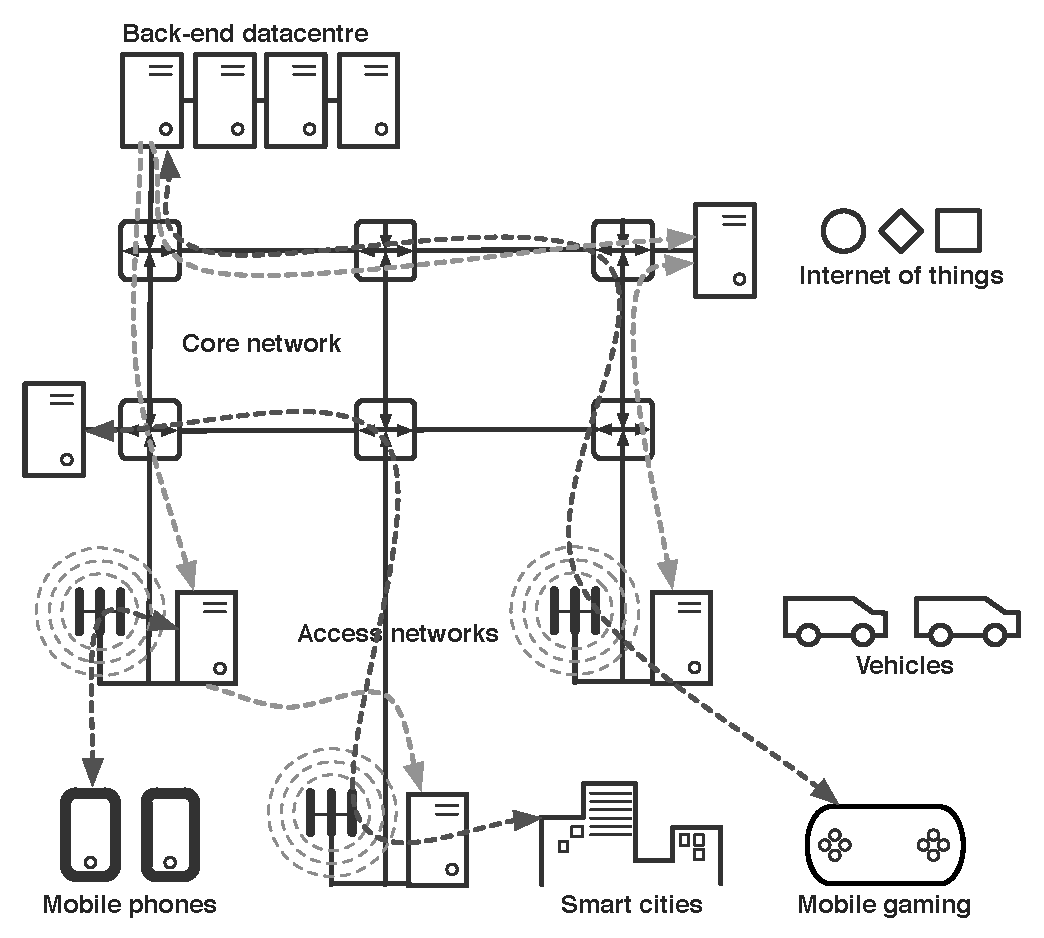
\includegraphics[width=\linewidth]{diagram_overview.pdf} 
	\caption{\xcloud}
	\label{fig:diagram_overview}
\end{figure}

\section{The case for the \xcloud}

\begin{itemize}
\item Internet structure, latency, and bandwidth: \cite{Ramasubramanian:2009:TIL:2492101.1555357}
\end{itemize}

\subsection{The bandwidth case for \xcloud}

\subsection{The latency case for \xcloud}
The intermediate latency between a client and a data centre is a product of propagation, modulation, and network routing and traffic shaping. Propagation is a clear physical obstacle to reducing latency, and there is very little evidence to suggest that information will propagate faster than $\frac{2}{3}$ of the speed of light, at scale, in the near future. Furthermore, the delay in the backbone network is incurred to the most part by routing. A full point to point network where the propagation speed is the only limit, is not economically viable and would dissolve the fabric of the Internet. As such, we can always expect a certain amount of network contributed latency and jitter. At best, an LTE mobile access network adds about 5 ms of latency \cite{blajic2006latency}. Radio access network latency can be expected to diminish over the next few generations of mobile networks. 

\begin{figure}[tb]
	\centering
	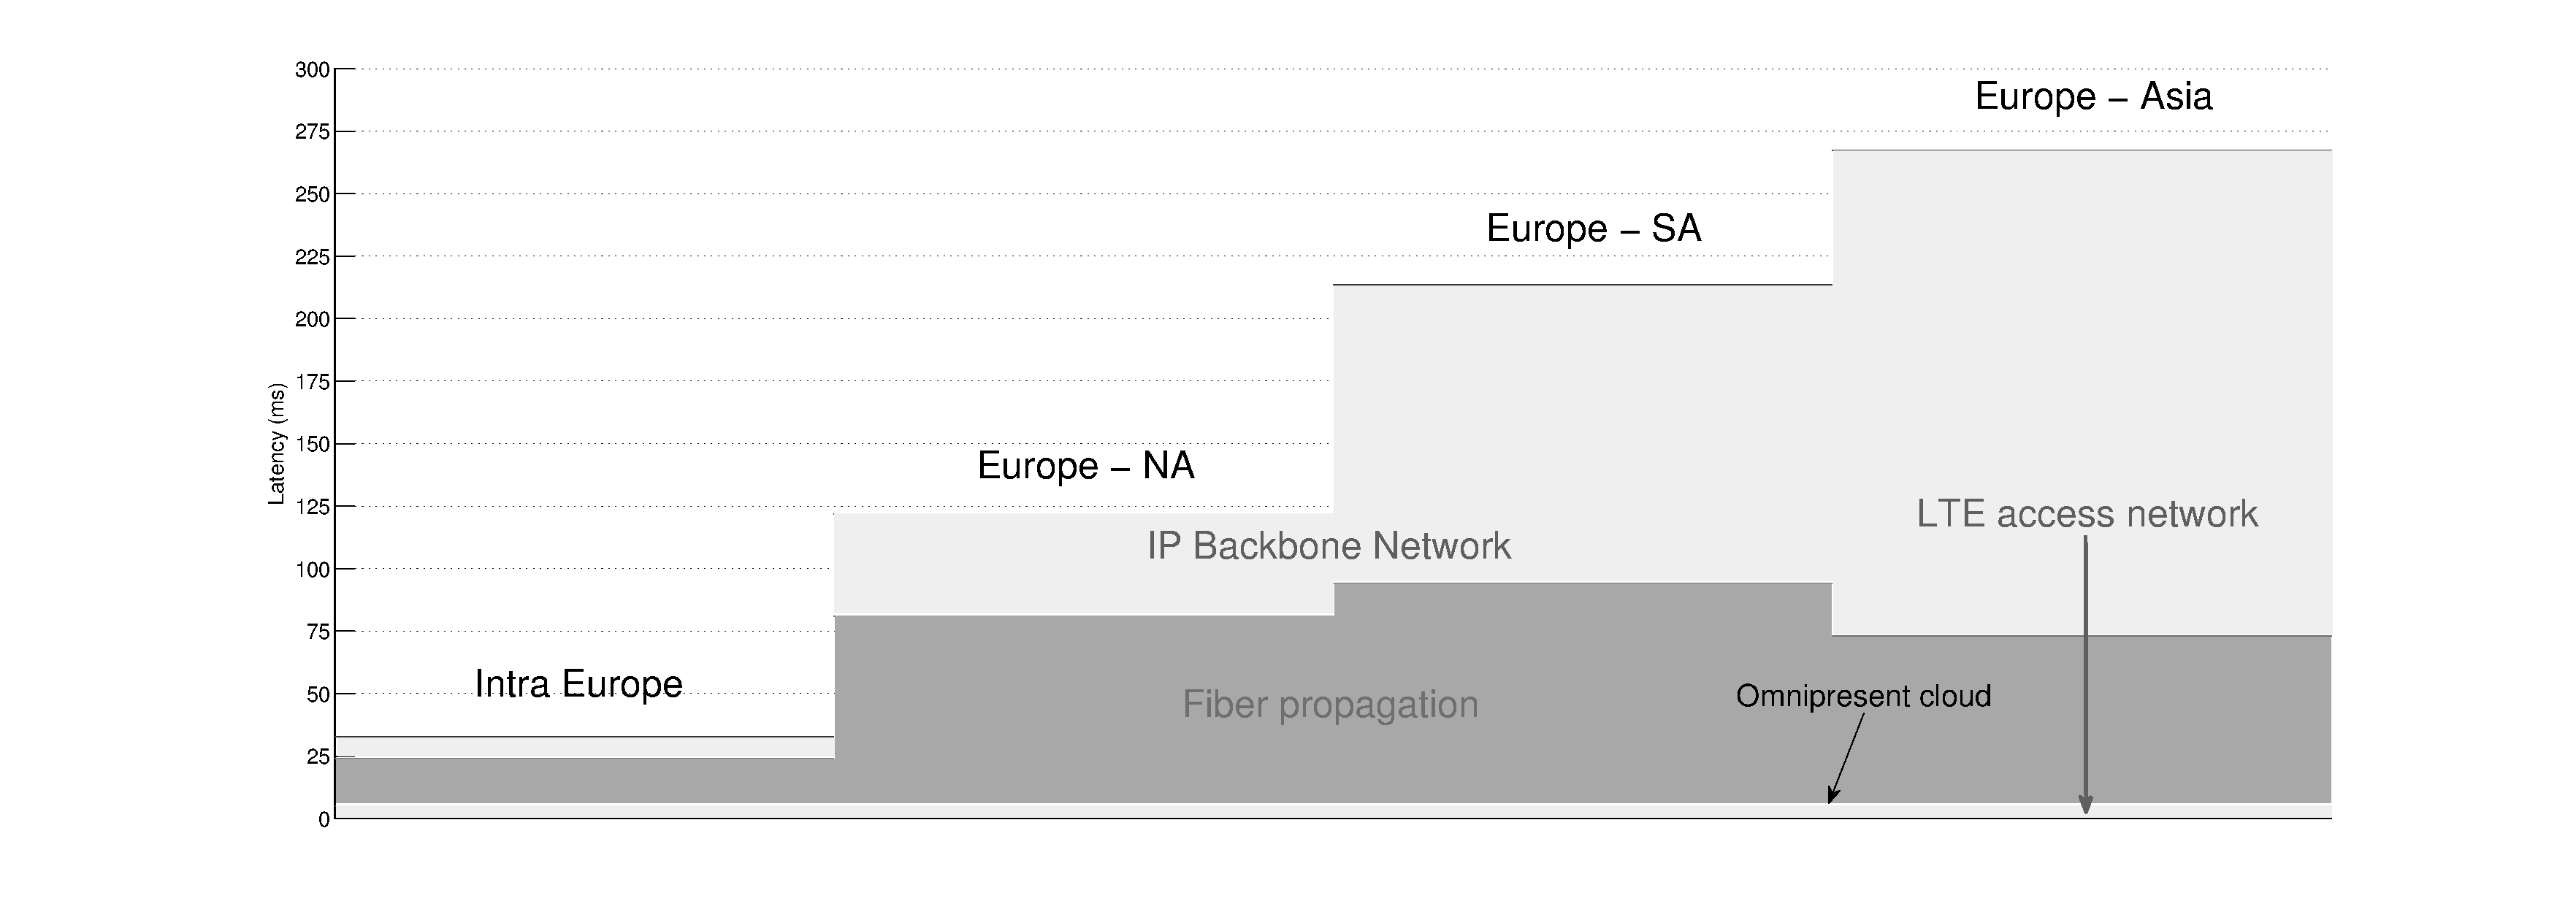
\includegraphics[height=0.12\paperheight]{omni_motivation.pdf} 
	\caption{IP Internet latency in western Europe \cite{BT_IP} over LTE \cite{blajic2006latency}}
	\label{fig:omni_motivation}
\end{figure}

Moving the cloud data centres closer to the IP backbone networks eliminates some of the additive latency on one side of the connection. Doing so, not only eliminate the propagation delay, but will over time, add more complexity to peripheries of the backbone as more severs nodes make their home there. 

The \xcloud remedies this latency challenge in a more sustainable way. By moving compute resources to the mobile networks, IP backbone network propagation and routing delays are eliminate without disrupting the Internet topology. The resulting distributed infrastructure is capable of delivering content and services at latencies less than 10 ms. 

The \xcloud will thus enable latency-sensitive services to be migrated to the cloud, such as, gaming, financial trading, process control, and most real-time human-machine interaction process.

\subsection{The infrastructure case for \xcloud}
Distributed virtualized mobile networks will rely on centralized compute nodes for higher level link management. One node will proposedly host multiple base stations, to which they connect over a network link, much like the Ericsson Radio Dot System \cite{ericsson_dot}, but at a larger scale. The size of these virtualization resource nodes is proportional to the maximum distance they can reside from the radio nodes, given the induced propagation delay. Supposedly these virtualization resource nodes will the placed in the vicinity of the core IP network. The virtualization resource nodes can be seen as to define geographic areas whos boundaries are defined by the reach of the mobile network which it serves. Depending on the level of desired provision and load balancing flexibility, these geographic domains will overlap to varying degrees.

The virtualization resource nodes are conceivably constructed of generic x86 or ARM servers, hosting VMs or containers within which the virtualized mobile network infrastructure is executed. Given the placement of the virtualization resource node, any free or designually excess capacity can be used hist other services.

The topology is designed to optimize the use of radio resources, the geographic domains which the virtualization resource nodes constitute do not necessarily overlap or map the demographic area which \xcloud services operate.

\section{Simulation model}

\subsection{Models}

\subsubsection{Data Centre}
\cite{5959161}

\subsubsection{Network}
\begin{itemize}
\item Latency
\begin{itemize}
\item "Point-to-Point" core network delay model \cite{choi2007analysis}
\item "One-hop" core network router queue delay model  \cite{papagiannaki2003measurement}
\end{itemize}
\end{itemize}

\subsection{Python + [NS-3, Omnet, Matlab, Modelica]}

\subsection{Java}

\section{Papers}

\subsection{Comparison of existing simulators from the perspective of  \xcloud}
A survey of existing simulators with comparison of their capabilities (and limitations) to simulate \xcloud.

Simulators of:
\begin{itemize}
\item Data centers,
\item BTS,
\item Network (BTS --- DC),
\item Mobile network,
\item Mobile devices,
\item Users (mobility).
\end{itemize}

What is different in operation/simulation of \xcloud?

\subsection{Limitations of current infrastructure \& the setup/structure of \xcloud}
\subsubsection{Limitations of current infrastructure}
Simulate the current infrastructure (mobile network + remote/big data centers) and show the limits of it.
\begin{itemize}
\item What will happen when the number of mobile devices increases by order(s) of magnitude? The influence on a network connection between a base station and a big/remote data center.
\item How many mobile devices can be handeled by the current infrastructure (depending on a latency limits)?
\end{itemize}
\subsubsection{The setup/structure of \xcloud}
The \xcloud consists of antennas, small (edge) data centers and big (remote) data centers.
Small data centers are located close to the antennas and can host both virtualized base station software and VMs with applications.
Big data centrs are located far away from users.
Small data centers have smaller amount of resources than big ones (maybe also performance is lower) and running applications there is more expensive.
However, latency is is much lower than in a case of big (remote) data centers.

Questions about the setup/structure of \xcloud:
\begin{itemize}
\item how many antennas should be associated with one small (local) data center? (probably this will be limited by the latency between an antenna and a small data center)
\item how big should small (local) data centers be (\#CPUs etc)?
\end{itemize}

\subsection{\xcloud model}

\subsection{Throughput and bandwidth limitations in the \xcloud}

\subsection{Virtual Machine placement and migration in \xcloud}

Regarding placement of Virtual Machines (VMs) in the edge data centers:
\begin{itemize}
\item Should a VM that serves all users (even these outside of the range of the directly connected antennas) be placed in an edge data cener or should it be rather an additional instance that serves users that are in the close proximity (duplicating a VM in a big data center)?
\item When a VM should be placed/duplicated in a small data center?
\item While users are moving from one antenna to another when VM should be migrated from one edge data center to another one?
\end{itemize}

\subsection{Other thoughts} 

\begin{itemize}
\item Different workload patterns?
\item How to perform monitoring? (System is very distributed)
\item Maybe new metrics to monitor (eg. distance from antenna, velocity, direction, etc.)
\item Changes in the architecture of mobile applications
\end{itemize}

\section{Conclusion}


\bibliographystyle{plain}
\bibliography{references}

\end{document}